\subsection{Struktur}

Da einige Aspekte in der Literatur zum Teil zusammen dargestellt wurden, sind diese auch im Modell hierarchisch angeordnet. Außerdem orientiert sich die Struktur der Übersicht über die Aspekte von Erklärbarkeit an dem Prinzip von Qualitätsmodellen wie es \citeauthor{schneider2012abenteuer} beschreibt \cite{schneider2012abenteuer} (Mehr siehe \autoref{sec:basics_quality_models}). Dabei werden abstrakte Ziele immer konkreter gefasst bis sie schlussendlich mit konkreten Metriken messbar sind. Das zugrunde liegende Modell (\glqq Goal-Driven and Property-Based Definition Approach for Product Metrics\grqq{} \cite{briand1995goal}) von \citeauthor{briand1995goal} definiert außerdem unter anderem die nötigen Abhängigkeiten von äußeren Faktoren, die hier dem bereits erwähnten \textit{Context} entsprechen. Da die Metriken der Evaluation zum Teil von den entwickelten Erklärungen abhängen, müssen die Eigenschaften im Gegensatz zu dem erwähnten Modell von \citeauthor{schneider2012abenteuer} allerdings zuerst definiert werden. Anderenfalls wäre es nicht möglich, Metriken zu entwickeln, welche direkt die Eigenschaften der Erklärungen messen. Metriken, welche der Messung von Auswirkungen von integrierten Erklärungen in einem System dienen, können allerdings bereits zuvor aufgestellt werden. Für die Formalierung des Messkonzeptes werden laut \citeauthor{briand1995goal} außerdem vorhande Abstraktionen benötigt. Als Artefakt sollen hier die Ausprägungen der Kategorie \textit{Evaluation} in \autoref{sec:model_evaluation} dienen.

\smallbreak

Aus vorherigem folgend werden die Punkte \textit{Context} und \textit{Objective} aus \autoref{tab:model_explaination_aspects} werden daher unter \textit{External Dependencies} zusammengefasst. Dies verdeutlicht, dass die \textit{Objectives} für das Integrieren von Erklärungen stark mit anderen äußeren Einflüssen (\textit{Context}) zusammenhängen (\autoref{sec:model_external_dependencies}).

Auch werden \textit{Demand}, \textit{Content} und \textit{Presentation} vereint, da sich diese drei Kategorien direkt auf die Eigenschaften von Erklärungen beziehen: \textit{Characteristics}. Damit wird der starke Zusammenhang zwischen den verschiedenen Merkmalen einer Erklärung deutlich.

\smallbreak

Folglich ist die Übersicht in die drei Kategorien \textit{External Dependencies}, \textit{Characteristics} und \textit{Evaluation} gegliedert, welche aufgrund der vorherigen Argumentation in dieser Reihenfolge in der Übersicht dargestellt sind. Ein Überblick ist in \autoref{fig:model_overview} zu sehen.

In den folgenden Abschnitten werden die Ausprägungen der einzelnen Kategorien sowie deren Anwendung in der Literatur beschrieben.

\begin{figure}[htb!]
    \begin{center}
        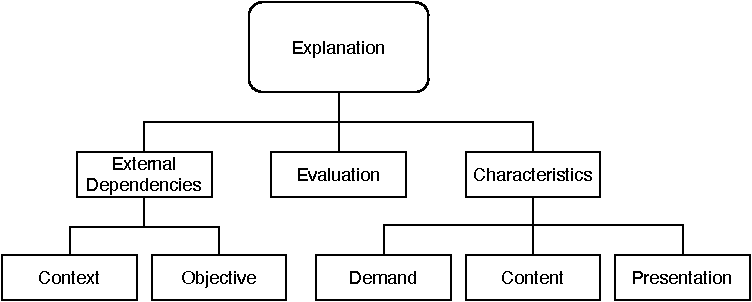
\includegraphics[width=0.9\linewidth]{contents/05_model_description/res/model-overview.pdf}
    \end{center}
    \caption{Oberkategorien der Aspekte von Erklärungen}
    \label{fig:model_overview}
\end{figure}